% ============================================================================
% Supplementary Material for STITCH_EXT_v9.tex (reSTITCHing)
% ----------------------------------------------------------------------------
% Compiles on its own (pdflatex / Overleaf / Tectonic) with figures/ next to it.
% ASCII only, no em-dashes. Sections S1..S9 are cited from the main text as
% "Supplementary Material Sn". Sources of every number: V9_CHANGES.md.
% Generated inputs: numbers_set4.tex, tables_set4.tex
%   (python -B phase2/frontier/make_numbers_set4.py).
% S8 is the Phase 3 write-up formerly in PHASE3_MPSOC_v2.tex, updated (Gemini
% ladder row, "loop-clean" naming).
% ============================================================================
\documentclass[11pt]{article}

\usepackage[margin=1in]{geometry}
\usepackage{booktabs}
\usepackage{tabularx}
\usepackage{graphicx}
\usepackage{xcolor}
\usepackage{enumitem}
\usepackage{amsmath}
\usepackage{hyperref}
\hypersetup{colorlinks=true, linkcolor=blue!50!black, urlcolor=blue!50!black, citecolor=blue!50!black}
\graphicspath{{figures/}}
% GENERATED by phase2/frontier/make_numbers_set4.py -- do not edit by hand.
% Re-run analysis_set4.py / analysis_set4b.py, then this script, to refresh.
\newcommand{\SetFourRuns}{612}  % set4_analysis.json runs_total
\newcommand{\SetFourErrored}{0}  % set4_analysis.json runs_errored
\newcommand{\SetFourPooledBase}{99.3}  % pass_rates pooled|baseline
\newcommand{\SetFourPooledBaseK}{152/153}  % pass_rates pooled|baseline
\newcommand{\SetFourPooledAdv}{98.7}  % pass_rates pooled|sem_adv
\newcommand{\SetFourPooledAdvK}{151/153}  % pass_rates pooled|sem_adv
\newcommand{\SetFourPooledEsc}{98.0}  % pass_rates pooled|sem_escalate
\newcommand{\SetFourPooledEscK}{150/153}  % pass_rates pooled|sem_escalate
\newcommand{\SetFourPooledRestart}{98.0}  % pass_rates pooled|sem_escalate_restart
\newcommand{\SetFourPooledRestartK}{150/153}  % pass_rates pooled|sem_escalate_restart
\newcommand{\SetFourGPTBaseK}{50/51}  % pass_rates gpt-4.1-mini-2025-04-14|baseline
\newcommand{\SetFourGPTToolRed}{70.5}  % tools gpt-4.1-mini-2025-04-14 reduction_pct
\newcommand{\SetFourGeminiBaseK}{51/51}  % pass_rates gemini-2.5-flash|baseline
\newcommand{\SetFourGeminiToolRed}{100.0}  % tools gemini-2.5-flash reduction_pct
\newcommand{\SetFourHaikuBaseK}{51/51}  % pass_rates claude-haiku-4-5-20251001|baseline
\newcommand{\SetFourHaikuToolRed}{96.5}  % tools claude-haiku-4-5-20251001 reduction_pct
\newcommand{\SetFourGPTDeltaAdv}{$-$2.0}  % contrasts gpt-4.1-mini-2025-04-14|sem_adv
\newcommand{\SetFourGPTDeltaEsc}{$-$3.9}  % contrasts gpt-4.1-mini-2025-04-14|sem_escalate
\newcommand{\SetFourGPTDeltaRestart}{$-$3.9}  % contrasts gpt-4.1-mini-2025-04-14|sem_escalate_restart
\newcommand{\SetFourMinP}{1.000}  % contrasts, min sign-flip p over all scopes and conditions
\newcommand{\SetFourToolRed}{88.6}  % tools pooled reduction_pct
\newcommand{\SetFourToolAdv}{2.29}  % tools pooled sem_adv
\newcommand{\SetFourToolEsc}{0.26}  % tools pooled sem_escalate
\newcommand{\SetFourInrPassMin}{0.11}  % cost, min inr_per_pass over model x condition
\newcommand{\SetFourInrPassMax}{0.51}  % cost, max inr_per_pass over model x condition
\newcommand{\SetFourFingerprintMain}{256}  % fingerprint_counts fp_b43877da5b
\newcommand{\SetFourFingerprintOther}{7}  % fingerprint_counts fp_6050bec882
\newcommand{\SetFourParitySim}{140/140}  % parity_check_osscad.json a_agree/candidates
\newcommand{\SetFourParityInterp}{51/51}  % parity_check_osscad.json b_agree/b_checked
\newcommand{\SetFourBPlanned}{228}  % 19 modules x 4 conditions x N=3
\newcommand{\SetFourBGPTValid}{228}  % set4b_analysis.json coverage gpt-4.1-mini-2025-04-14 valid
\newcommand{\SetFourBGPTErrored}{0}  % coverage gpt-4.1-mini-2025-04-14 errored
\newcommand{\SetFourBGeminiValid}{228}  % set4b_analysis.json coverage gemini-2.5-flash valid
\newcommand{\SetFourBGeminiErrored}{0}  % coverage gemini-2.5-flash errored
\newcommand{\SetFourBHaikuValid}{143}  % set4b_analysis.json coverage claude-haiku-4-5-20251001 valid
\newcommand{\SetFourBHaikuErrored}{85}  % coverage claude-haiku-4-5-20251001 errored
\newcommand{\SetFourBHaikuPending}{85}  % planned - Haiku valid
\newcommand{\SetFourBValidTotal}{599}  % coverage, sum of valid runs
\newcommand{\SetFourAllValid}{1211}  % Set 4 valid runs + Set 4b valid runs
\newcommand{\SetFourBFloorModules}{19}  % Q1 modules
\newcommand{\SetFourBLeaveFloor}{16}  % Q1: modules with a non-floor baseline tier for at least one model
\newcommand{\SetFourBCeilingAll}{4}  % Q1: modules at ceiling for all three models
\newcommand{\SetFourBStillFloor}{\texttt{adder\_pipe\_64bit}, \texttt{alu} and \texttt{freq\_divbyfrac}}  % Q1: floor for every model that ran them
\newcommand{\SetFourBToolFails}{188}  % Q2: fails in the three tool conditions
\newcommand{\SetFourBToolFailsSF}{103}  % Q2: of those, with semantic_fired
\newcommand{\SetFourBToolFailsSFPct}{55}  % Q2: percentage
\newcommand{\SetFourBDBPZeroCells}{3}  % Q2: passes with a directive before the pass in baseline-0/3 cells (all traced, none attributable)
\newcommand{\SetFourBMinP}{0.062}  % Q3: min sign-flip p
\newcommand{\SetFourBQThreeContrasts}{12}  % Q3: number of contrasts
\newcommand{\SetFourBAllThreeModules}{12}  % Q4: modules every model ran
\newcommand{\SetFourBQFour}{\texttt{freq\_divbyfrac}}  % Q4 strict list
\newcommand{\SetFourBQFourRuns}{36}  % Q4: valid runs on the strict module
\newcommand{\SetFourBAluGemini}{3/12}  % Q4_table alu gemini


\renewcommand{\thesection}{S\arabic{section}}
\renewcommand{\thetable}{S\arabic{table}}
\renewcommand{\thefigure}{S\arabic{figure}}
\setlist{itemsep=0.1em, topsep=0.25em, leftmargin=1.2em}
\newcommand{\cond}[1]{\texttt{#1}}
\newcommand{\fitbox}[1]{\resizebox{\ifdim\width>\linewidth\linewidth\else\width\fi}{!}{#1}}

\title{\textbf{Supplementary Material}\\[4pt]
\large\textnormal{reSTITCHing: Replicated, Cost-Controlled, and Sign-off-Aware Repair of LLM-Generated RTL}}
\author{Karthikeya Patana \and Yashwant Rajesh \and Aathira Sunil \and Durga Saranyu \and Sri Parameswaran \and Kamesh Chandrasekar \and Paresh Saxena \and Soumya Joshi}
\date{}

\begin{document}
\sloppy
\maketitle
\tableofcontents

% ============================================================================
\section{Interpreter, Conditions and Escalation}
\label{s:interp}

\textbf{Production interpreter (v2).} \texttt{src/interpreter/stitch\_interpreter.py},
never edited since Phase~2 (SHA-256 of the LF-normalised file
\texttt{42f61a49\ldots2abff}, recorded in every Phase~3 run). Table~\ref{tab:s-rules}
lists its classes with their verification status.

\begin{table}[htbp]
\centering
\caption{Interpreter classes and whether each was verified against real tool
output (not only synthetic strings). Phase~3 status from the MPSoC logs.}
\label{tab:s-rules}
\small
\begin{tabularx}{\linewidth}{@{}l l X@{}}
\toprule
\textbf{Class} & \textbf{Source} & \textbf{Verified on real data} \\
\midrule
\cond{UNUSEDSIGNAL} & Verilator & yes, two modules and two models (the replicated illustrations); wrong directive on clock ports and on partially used buses (Phase~3) \\
\cond{MULTIDRIVEN} & Verilator & yes, both Verilator~5 message formats; first net only \\
\cond{UNDRIVEN} & Verilator & synthetic plus one real regression case \\
\cond{WIDTHTRUNC}/\cond{WIDTHEXPAND} & Verilator & yes for named operands; silently dropped when the operand is an expression \\
\cond{BLKSEQ} & Verilator & yes; signal extraction yields a prose word on Verilator~5 output \\
\cond{COMBDLY} & Verilator & real Verilator~5 uses the code for \texttt{<=} in a combinational block, not a \texttt{\#} delay; the template assumes the latter \\
Latch inferred & Yosys & yes \\
Combinational loop & Yosys & yes; a loop reported only by Verilator (\cond{UNOPTFLAT}) is missed \\
\midrule
\cond{MISSING\_CLOCK} (v3) & fusion & yes, two MPSoC router registers \\
\cond{ASYNC\_RESET} (v3) & Yosys & yes, the one-bit router register that aborts synthesis \\
\cond{COMB\_LOOP} (v3) & Verilator & yes, an instruction-fetch loop \\
\cond{WIDTH\_EXPR} (v3) & Verilator & yes, the flit packer \\
\cond{PINMISSING} (v3) & Verilator & yes ($748$ in the MPSoC); composition-level, not a repair task \\
\cond{RESET\_UNUSED} (v3) & Verilator & synthetic only \\
\bottomrule
\end{tabularx}
\end{table}

\textbf{v3 layer.} \texttt{src/interpreter/stitch\_interpreter\_v3.py} (version
$3.0.1$ in every Phase~3 run) imports v2 unchanged; \texttt{interpret(...,
version="v2")} reproduces v2 byte for byte, and tests enforce it. It caps its
output at three directives, suppresses the gating template on clock ports and
on partially used buses, routes advice to the right module in multi-module
files, and adds the classes above.

\textbf{Conditions.} \cond{baseline}: simulation log only. \cond{raw\_adv}:
plus the filtered raw Verilator and Yosys lines. \cond{sem\_adv}: plus the
interpreter's directives on every iteration. \cond{sem\_escalate}: starts as
\cond{baseline}; after $N{=}2$ consecutive failures with the same error
signature it escalates permanently to the \cond{sem\_adv} feedback.
\cond{sem\_escalate\_restart}: as \cond{sem\_escalate}, plus one blank-slate
prompt after $M{=}3$ consecutive same-signature failures counted from the first
escalated iteration (the triggering failure is not counted); the streak then
resets and the run stays escalated. The signature keys on the first $5$ lines of
the normalised log. The state for iteration $i$ is decided from iterations
$1$ to $i{-}1$ only, so the iteration whose failure triggers escalation still
ran under baseline tooling. The state machine is a pure class with unit tests
(\texttt{phase1/escalation\_state.py}). Phase~3 adds \cond{baseline\_gate}
and the gate message (Section~\ref{s:p3}).

% ============================================================================
\section{Replication Details}
\label{s:replication}

\textbf{The two illustrations.} In \texttt{decoder\_3to8} and \texttt{mux4\_oe}
the model omits a declared gating port (\texttt{enable}, \texttt{oe}) on
iteration one; Verilator fires \cond{UNUSEDSIGNAL}; the directive resolves the
module in two iterations against a six-iteration failure for both controls on
gemma3:4b. On those enabling cells the interpreter also cuts token cost roughly
$5$ to $7\times$ against both controls. The survivors are small, but primitives
compose: a forgotten output-enable on a multiplexer instantiated many times in
a design is that many latent defects, and the MPSoC study tests exactly this
argument.

\begin{table}[htbp]
\centering
\caption{The reachability check: forgotten inputs are reachable, forgotten
outputs are not (gemma3:4b, hand-built diagnostic modules, not RTLLM).
\texttt{sf} = \cond{semantic\_fired}.}
\label{tab:s-asym}
\small
\begin{tabular}{@{}l l l c@{}}
\toprule
\textbf{Target class} & \textbf{Module} & \textbf{Iteration-1 behaviour} & \textbf{sf} \\
\midrule
Forgotten input  & decoder\_3to8 & port declared, never read & $1$ \\
Forgotten input  & mux4\_oe      & \texttt{oe} never referenced & $1$ \\
Forgotten output & adder\_with\_overflow & output assigned unprompted & $0$ \\
Forgotten output & fsm\_next\_state\_error & output assigned on all paths & $0$ \\
\bottomrule
\end{tabular}
\end{table}

\textbf{Retirements.} \texttt{datapath\_mux\_alu}/llama3.1 passed
\cond{sem\_adv} in $2$ of $3$ samples with \cond{semantic\_fired}${=}0$ in all
three; \texttt{instr\_decode\_unit}/gemma3:4b fired \cond{UNUSEDSIGNAL}
correctly and still failed, regressing into an unrelated syntax loop; and
\texttt{alu\_with\_enable} became too easy after redesign. Several further
candidates built to elicit the gated-input defect were discarded because the
specification accidentally handed the model the answer, or because the defect
was a missing default the system prompt already forces.

\textbf{The in-house benchmark.} The $255$-run benchmark was built from
historical $N{=}1$ labels. Re-measured at $N{=}3$, $4$ of $5$ ``real-test'' and
$2$ of $3$ ``enabling'' cells do not reproduce the baseline behaviour their
category was defined by. The regression gate held: both replicated
illustrations pass $4/4$ on strict pass/fail under the new conditions.

% ============================================================================
\section{Harness Defects}
\label{s:harness}

\textbf{Defect A (simulator working directory).} The simulation invocation set
no working directory, so any testbench doing relative-path file I/O
(\texttt{\$readmemh}) could never resolve its data file, whatever the generated
logic. It disqualified every file-I/O design and was confirmed not to affect the
conference benchmark.

\textbf{Defect B (unclosed code-fence extraction).} An unclosed
\texttt{```verilog} fence left the opening marker attached, corrupting
otherwise-compilable code: $58$ of $659$ generated files ($8.8\%$).

\textbf{Defect C (pass-string mismatch).} The harness checked for the
case-sensitive substring \texttt{"PASS"} or \texttt{"ALL TESTS PASSED"}; RTLLM
testbenches print \texttt{"Your Design Passed"}. A re-scan of $64$ completed
runs found $20$ ($31\%$) misclassified as failures, with corrupted trajectories:
a cell that passed on iteration one was told it failed and spent its remaining
iterations changing correct code.

The confirmatory harness routes every pass/fail decision through
\texttt{detect\_outcome(log, benchmark)}, backed by a per-benchmark registry;
the benchmark is a required argument with no default, so a new benchmark must
register its conventions and an unregistered one fails at import. It was
regression-verified against $64$ manually adjudicated cells before any full run.

% ============================================================================
\section{RTLLM Pool, Pilot and the Fine-Tuning Twin}
\label{s:twin}

\textbf{Pool.} RTLLM~v2.1 has $50$ designs; a batch compatibility screen found
$44$ compatible with the Icarus flow, and each of the $6$ exclusions has a
documented cause, one of them a defect in RTLLM's own reference.
\texttt{edge\_detect} and \texttt{square\_wave} were excluded because their
testbenches pass with stuck-at-$0$ outputs. $42$ modules remain.

\textbf{Pilot.} A five-module pilot completed three modules before a thermal
stop and showed no condition differentiation: they spanned a ceiling
(\texttt{counter\_12}), a floor (\texttt{accu}) and a flat mid-point
(\texttt{barrel\_shifter}), none in the band where an effect is measurable.
Hence the tiers.

\textbf{Twin design.} RTLCoder-Deepseek-v1.1 is fine-tuned from the
DeepSeek-Coder-6.7B base weights already in the study, so the pair isolates
fine-tuning. gemma3:4b and llama3.1 are ladder context; RTLCoder runs under its
native stub-completion prompt and under the shared harness prompt, so prompt
format is measured rather than confounded. $5$ model-conditions $\times 42$
modules $\times N{=}3 = 630$ pre-registered runs at $T{=}0.5$,
\cond{baseline} only; all completed with zero errors.

\textbf{Verdict.} On the $17$ recoverable modules ($51$ runs per
model-condition): deepseek-coder shared $32/51$ ($62.7\%$), RTLCoder native
$29/51$ ($56.9\%$), RTLCoder shared $21/51$ ($41.2\%$). At the shared prompt
RTLCoder wins $0$ modules, ties $13$ and loses $4$ ($|\Delta|\leq1$ as the tie
threshold, the $N{=}3$ noise floor); at the native prompt the comparison is a
wash ($5$ wins, $6$ ties, $6$ losses). The four shared-prompt losses trace to a
submodule-hierarchy mismatch, SystemVerilog dialect leakage, a parameter-binding
failure, and, on \texttt{fixed\_point\_substractor}, a naming artefact in which
RTLCoder reproduces RTLLM's folder name rather than the specified module name,
identically under both prompts. By functional class RTLCoder (native) clears
every recoverable signal-processing module ($9/9$, three modules) and the
recoverable memory module ($3/3$, \texttt{LFSR}), and scores $2/6$ on control
(two modules) where deepseek-coder scores $0/6$; across all $42$ modules the
native prompt is $9/15$ on signal processing and $6/12$ on memory. Prompt
format: native wins $3$ modules, shared $2$, $12$ tie, while in total native
passes $29/51$ against $21/51$ (Figure~\ref{fig:s-twin}).

\begin{figure}[htbp]
\centering
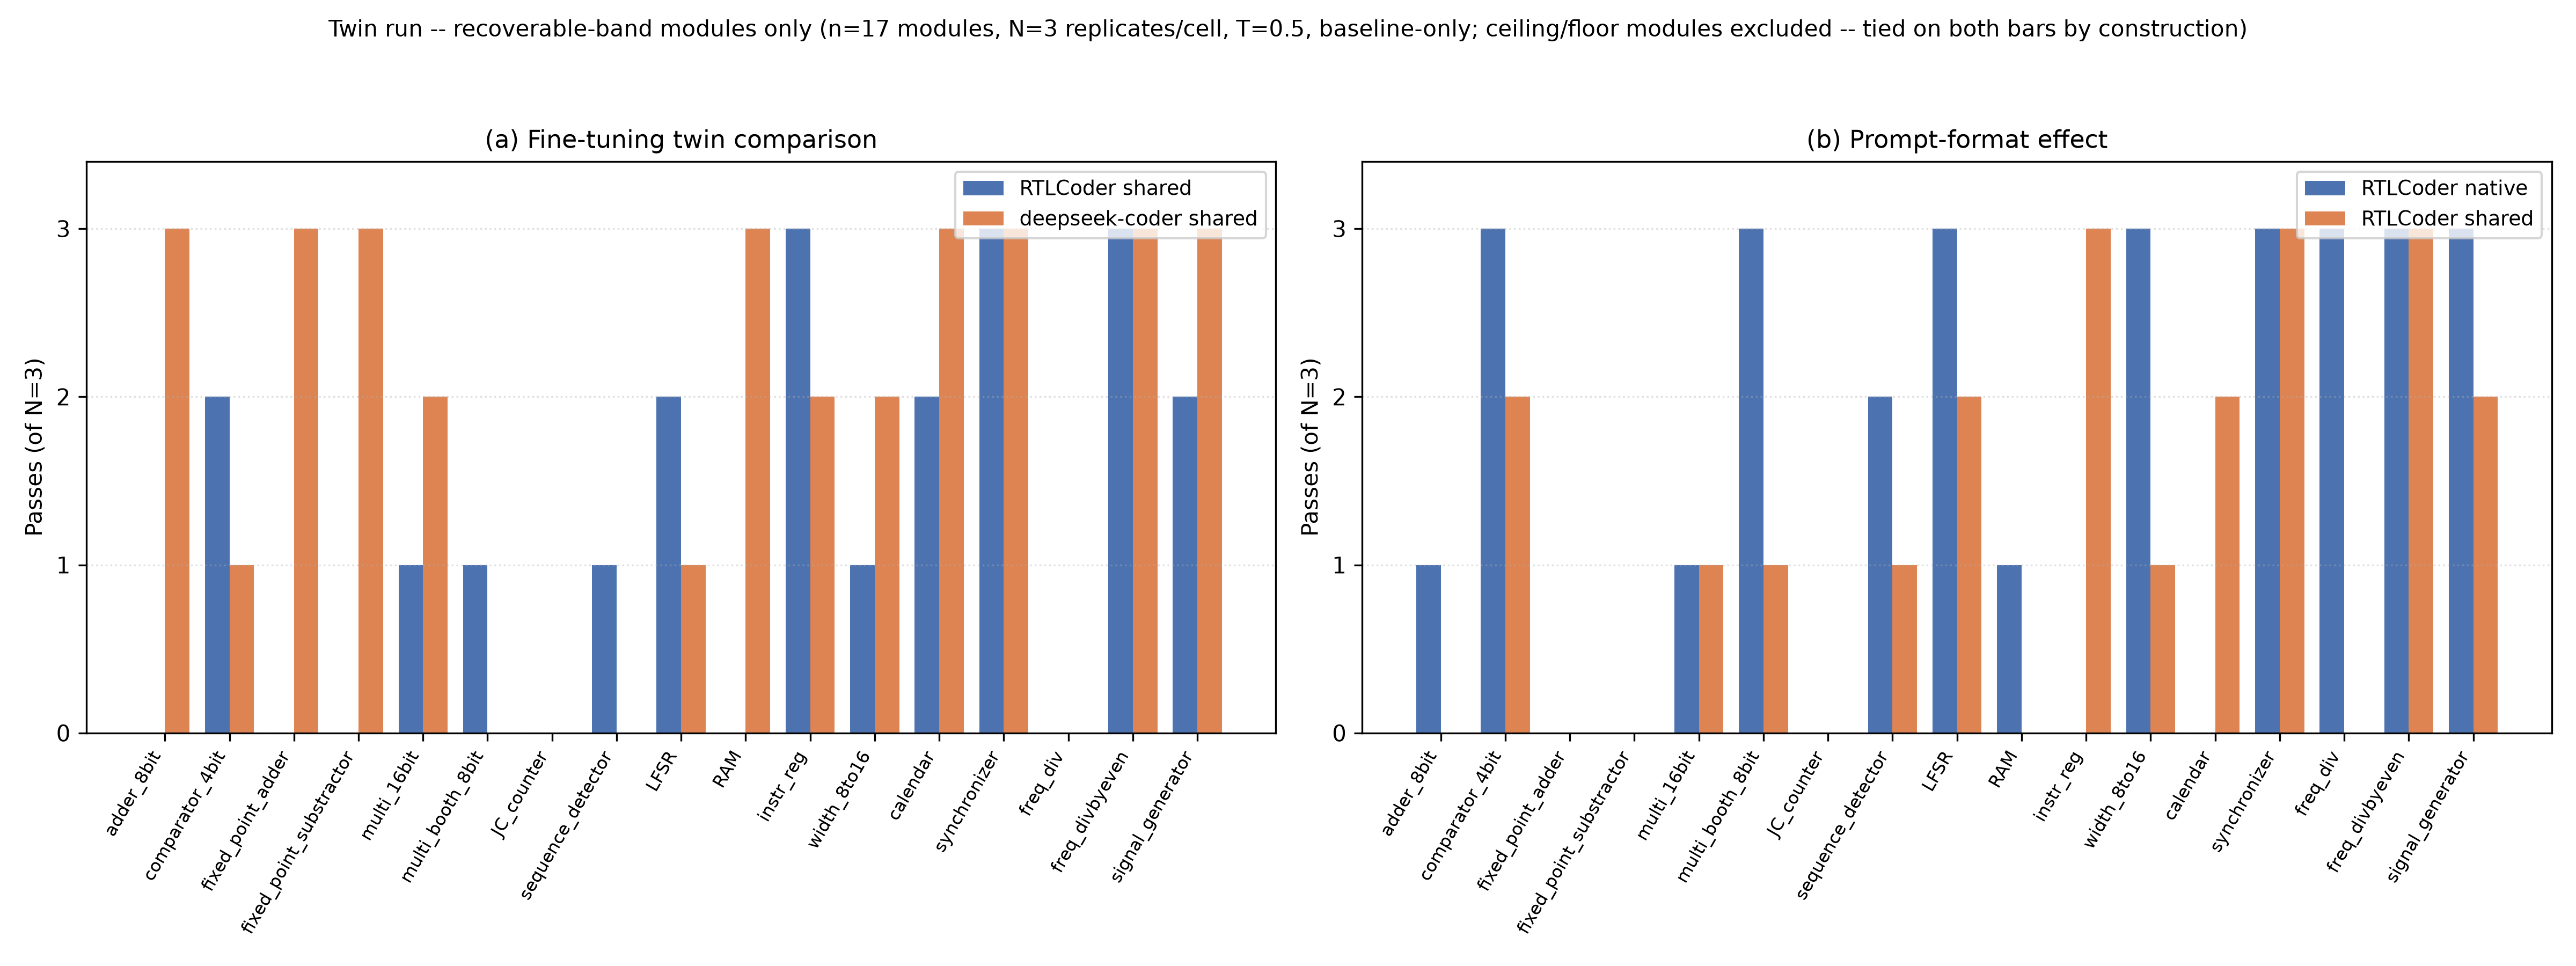
\includegraphics[width=\linewidth]{twin_named_comparisons.png}
\caption{(a) Fine-tuning twin: RTLCoder shared against deepseek-coder shared,
$17$ recoverable modules ($0$ wins, $13$ ties, $4$ losses: \texttt{adder\_8bit},
\texttt{fixed\_point\_adder}, \texttt{fixed\_point\_substractor}, \texttt{RAM};
\texttt{width\_8to16}, $1/3$ against $2/3$, counts as a tie). (b) Prompt
format: native against shared for RTLCoder; native wins $3$, shared $2$.}
\label{fig:s-twin}
\end{figure}

% ============================================================================
\section{Sets 1 and 3 in Detail}
\label{s:sets13}

\textbf{Scope and timeouts.} Set~1: of $1{,}512$ cells, $6$ ($0.4\%$) errored
as timeouts and are excluded: five on \texttt{RAM} with llama3.1
(\cond{sem\_escalate} replicates $1$ to $3$, \cond{sem\_escalate\_restart}
replicates $1$ and $3$) and one on \texttt{LIFObuffer} with deepseek-coder
(\cond{sem\_escalate\_restart}, replicate $2$). \texttt{RAM}/llama3.1 is $0/3$
under baseline and \cond{sem\_adv}, so counting the missing runs as failures
moves the recoverable rates to $47/153$ ($30.7\%$) and $54/153$ ($35.3\%$); no
conclusion changes. Set~3: of $612$ cells, $2$ ($0.3\%$) errored
(qwen2.5-coder:32b, one \texttt{comparator\_4bit} and one
\texttt{multi\_booth\_8bit}).

\textbf{Iteration budget.} \cond{baseline} and \cond{sem\_adv} were capped at
six iterations, the escalation policies at eight, the Twin baselines at eight.
On the recoverable band one \cond{sem\_escalate} and one
\cond{sem\_escalate\_restart} pass in Set~1 arrived only in iterations seven or
eight ($47/150$ becomes $46/150$, and $54/151$ becomes $53/151$, at a cap of
six), and none in Set~3; at an equal cap \cond{sem\_escalate\_restart} is
$53/151$ ($35.1\%$) against baseline's $54/153$ ($35.3\%$).

\begin{table}[htbp]
\centering
\caption{Set~1 passes by tier and condition ($3$ models $\times$ $N{=}3$).}
\label{tab:s-tier-pass}
\small
\begin{tabular}{@{}l c c c c c@{}}
\toprule
\textbf{Tier} & \textbf{Modules} & \cond{baseline} & \cond{sem\_adv} & \cond{sem\_escalate} & \cond{sem\_esc\_restart} \\
\midrule
Ceiling     & $6$  & $44/54$   & $44/54$   & $46/54$   & $43/54$ \\
Recoverable & $17$ & $54/153$  & $47/153$  & $47/150$  & $54/151$ \\
Floor       & $19$ & $11/171$  & $12/171$  & $11/171$  & $11/170$ \\
\midrule
Pooled      & $42$ & $109/378$ ($28.8\%$) & $103/378$ ($27.2\%$) & $104/375$ ($27.7\%$) & $108/375$ ($28.8\%$) \\
\bottomrule
\end{tabular}
\end{table}

\begin{table}[htbp]
\centering
\caption{Set~1 Verilator+Yosys invocations per run by tier; reduction of
\cond{sem\_escalate} against \cond{sem\_adv}.}
\label{tab:s-tier-cost}
\small
\begin{tabular}{@{}l c r r r@{}}
\toprule
\textbf{Tier} & \textbf{Modules} & \cond{sem\_adv} & \cond{sem\_escalate} & \textbf{Reduction} \\
\midrule
Ceiling     & $6$  & $4.02$ & $1.00$ & $75.1\%$ \\
Recoverable & $17$ & $6.74$ & $5.62$ & $16.6\%$ \\
Floor       & $19$ & $7.28$ & $6.54$ & $10.1\%$ \\
\midrule
Pooled      & $42$ & $6.60$ & $5.38$ & $18.5\%$ \\
\bottomrule
\end{tabular}
\end{table}

\begin{figure}[htbp]
\centering
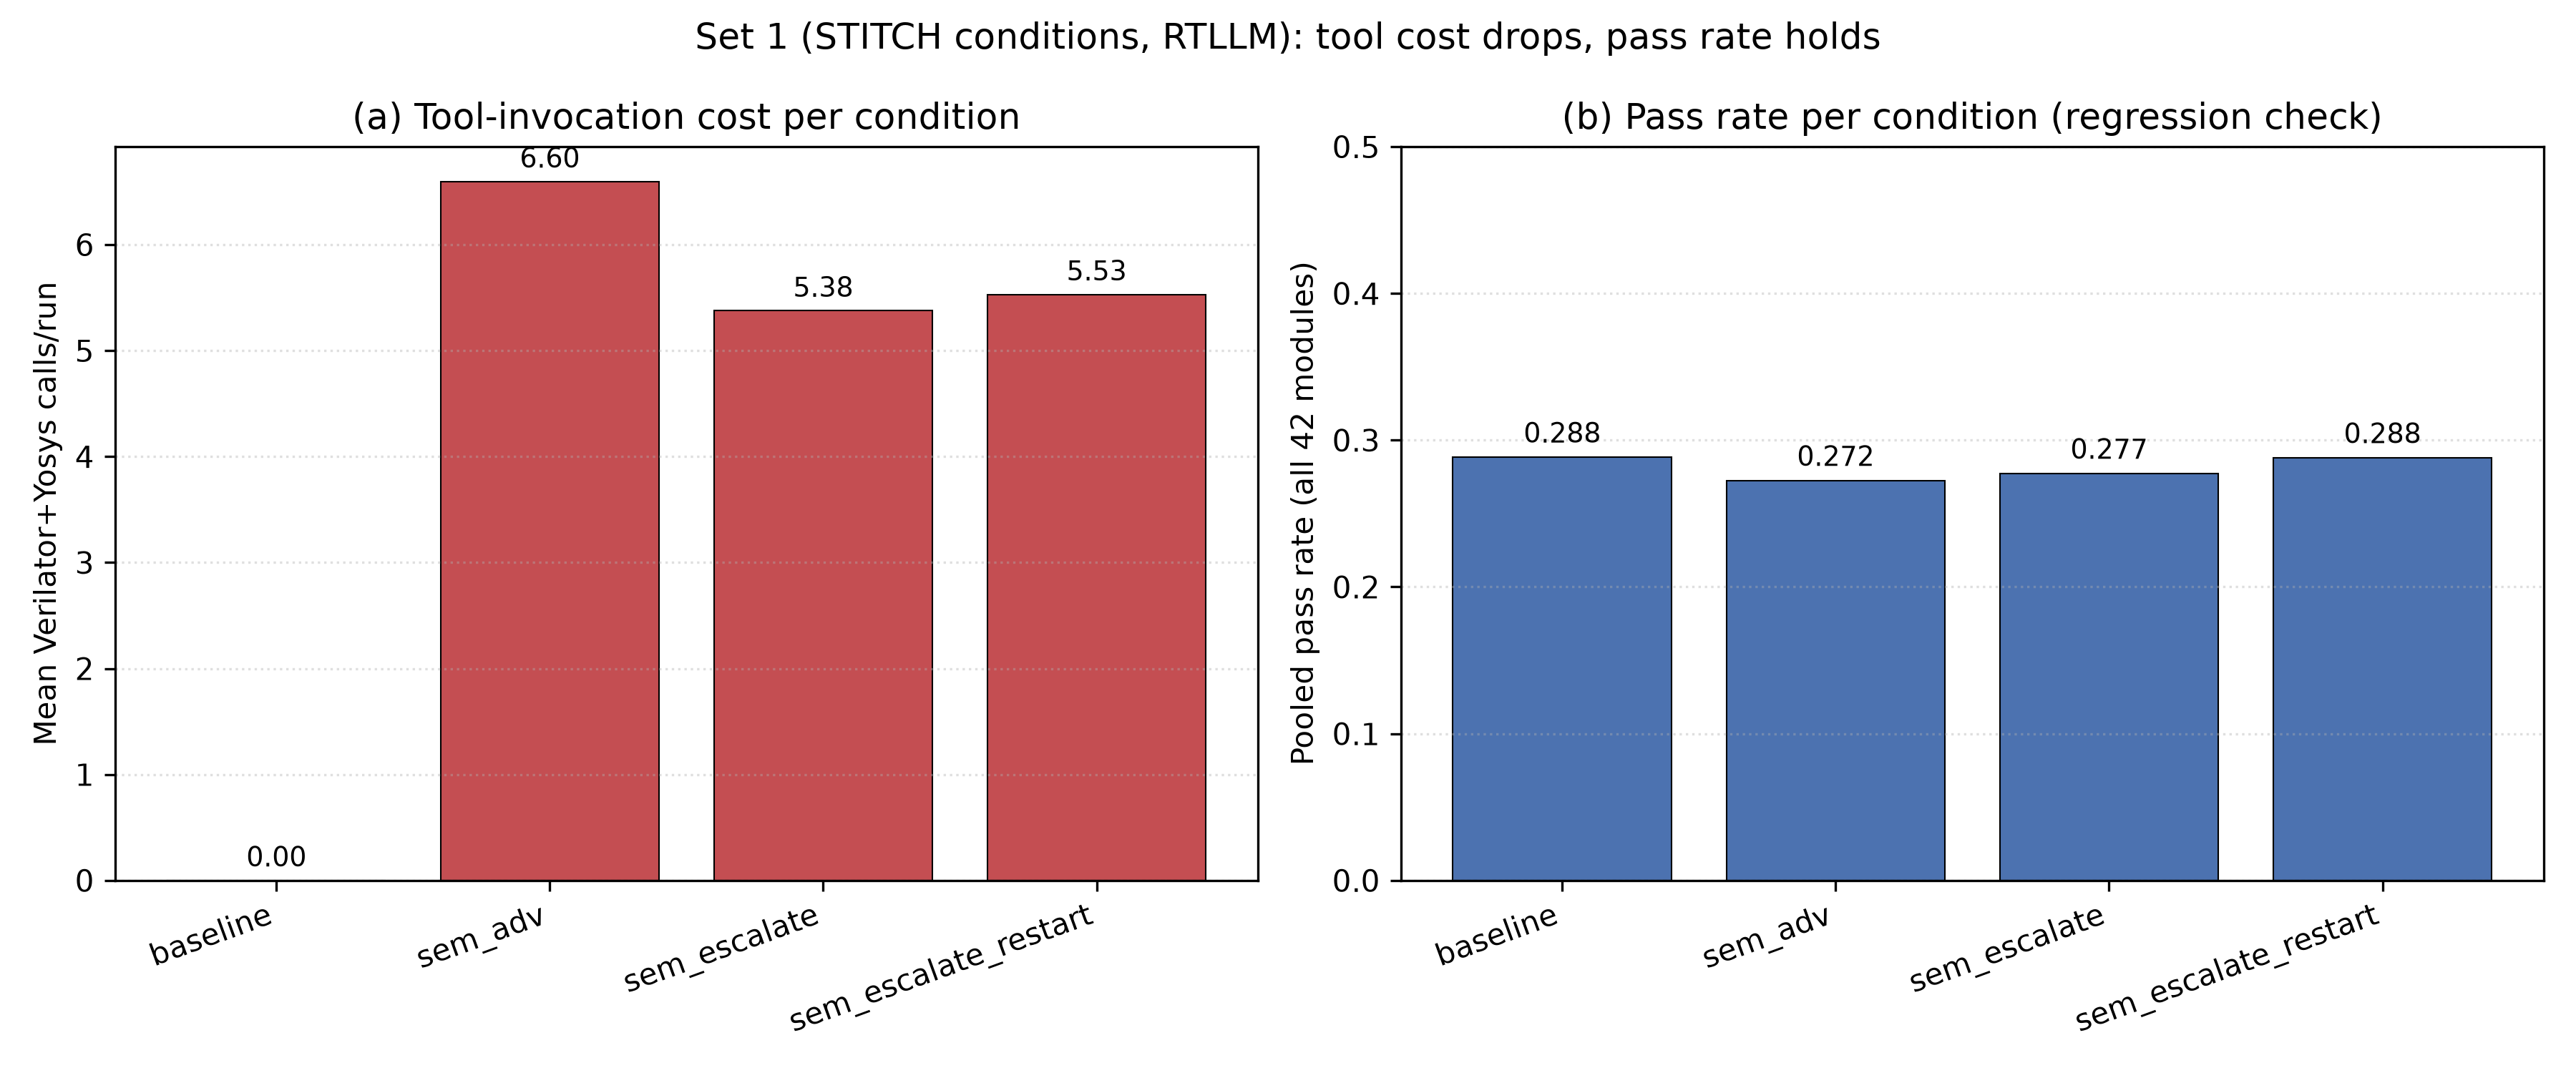
\includegraphics[width=0.9\linewidth]{set1_cost_passrate.png}
\caption{Set~1, $1{,}512$ runs: (a) Verilator+Yosys invocations per run by
condition, pooled; (b) pooled pass rate within $1.6$ points across conditions.}
\label{fig:s-set1-cost}
\end{figure}

\begin{table}[htbp]
\centering
\caption{Set~3, recoverable band, $T{=}0.1$: pooled and per model ($n{=}51$
per cell, except qwen2.5-coder:32b \cond{sem\_esc\_restart} $n{=}49$).}
\label{tab:s-set3}
\small
\begin{tabular}{@{}l c c c c@{}}
\toprule
\textbf{Model} & \cond{baseline} & \cond{sem\_adv} & \cond{sem\_escalate} & \cond{sem\_esc\_restart} \\
\midrule
qwen2.5-coder:14b & $52.9\%$ & $49.0\%$ & $56.9\%$ & $58.8\%$ \\
gemma3:27b        & $37.3\%$ & $45.1\%$ & $37.3\%$ & $33.3\%$ \\
qwen2.5-coder:32b & $78.4\%$ & $72.6\%$ & $82.4\%$ & $83.7\%$ \\
\midrule
Pooled            & $86/153$ ($56.2\%$) & $85/153$ ($55.6\%$) & $90/153$ ($58.8\%$) & $88/151$ ($58.3\%$) \\
\bottomrule
\end{tabular}
\end{table}

\textbf{Replicate trace (Set~3).} Of $153$ \cond{sem\_escalate} runs, $88$ passed
without escalating, $65$ escalated, and $2$ of those passed, both with
\cond{semantic\_fired}${=}0$, rescued by raw Verilator and Yosys feedback within
the first six iterations. No passing \cond{sem\_escalate} run had the interpreter
fire; for \cond{sem\_escalate\_restart} one of $88$ passing runs did, and seven of
\cond{sem\_adv}'s $85$. The net pooled escalation lead ($+4$ runs) comes from six
cells gaining seven runs in total against three cells losing one each. Set~3
tool calls on the recoverable band: $5.31$ (\cond{sem\_adv}) to $3.85$
(\cond{sem\_escalate}) per run, $27.6\%$.

\begin{table}[htbp]
\centering
\caption{Recoverable-band contrasts against baseline, (model, module) cell
bootstrap $95\%$ CI and sign-flip $p$ (\texttt{phase3/runner/posthoc\_checks.py}).}
\label{tab:s-posthoc}
\small
\begin{tabular}{@{}l l c c c@{}}
\toprule
\textbf{Run} & \textbf{Condition $-$ baseline} & \textbf{Passes} & \textbf{$\Delta$ [CI]} & \textbf{$p$} \\
\midrule
Set~1 & \cond{sem\_adv}              & $47/153$ vs $54/153$ & $-4.6$ [$-10.5$, $+0.7$] & $0.199$ \\
Set~1 & \cond{sem\_escalate}         & $47/150$ vs $54/153$ & $-4.7$ [$-10.7$, $+0.0$] & $0.148$ \\
Set~1 & \cond{sem\_escalate\_restart} & $54/151$ vs $54/153$ & $0.0$ [$-4.6$, $+4.6$]  & $1.000$ \\
Set~3 & \cond{sem\_adv}              & $85/153$ vs $86/153$ & $-0.7$ [$-7.8$, $+6.5$]  & $1.000$ \\
Set~3 & \cond{sem\_escalate}         & $90/153$ vs $86/153$ & $+2.6$ [$-1.3$, $+7.2$]  & $0.404$ \\
Set~3 & \cond{sem\_escalate\_restart} & $88/151$ vs $86/153$ & $+2.0$ [$-2.6$, $+7.2$]  & $0.596$ \\
\bottomrule
\end{tabular}
\end{table}

% ============================================================================
\section{The API Study (Sets 4, 4b and 4c)}
\label{s:api}

\textbf{Design.} Pre-registered in \texttt{phase2/frontier/SET4\_PREREG.md}
(original and five dated amendments, each hashed before the calls it governs;
hash after the last amendment \texttt{CC23711D\ldots653B}). Models:
\texttt{gpt-4.1-mini-2025-04-14} (pinned snapshot),
\texttt{gemini-2.5-flash} (\texttt{thinkingBudget} $0$) and
\texttt{claude-haiku-4-5-20251001} (no extended thinking), selected as the most
capable non-reasoning model per provider under a cost rule; $T{=}0.1$;
\texttt{max\_tokens} $8{,}192$. Any reasoning token or reasoning content on any
call stops the provider; there were none. The engine is the Set~3 runner with
only the model call replaced; pass detection is
\texttt{detect\_outcome(log, benchmark="rtllm")}. Toolchain: oss-cad-suite
20260917 in WSL, matched to the cluster build (Yosys~0.69+71, Verilator~5.053,
Icarus~14.0); on $140$ saved Set~3 candidates it reproduces the cluster verdicts
($\SetFourParitySim$ pass/fail, $\SetFourParityInterp$ interpreter outputs).
Every call logs provider-reported tokens, the returned model version, request
and response identifiers and cost; truncations: $0$ in every set.

\textbf{Deviations, disclosed.} (1) A fourth model (Kimi K2.6) stopped at its
smoke test with \texttt{reasoning\_tokens}${=}1$ and was dropped by decision; a
third ceiling model at a forced $T{=}0.6$ would add no information. (2)
OpenAI's \texttt{system\_fingerprint} changed during the run
($\SetFourFingerprintMain$ and $\SetFourFingerprintOther$ calls) for the same
snapshot. (3) Set~4b first stopped at caps set from a pilot projection that
underestimated floor cost; completion runs resumed from the master logs without
re-running any completed run. Claude Haiku~4.5 is at
$\SetFourBHaikuValid/\SetFourBPlanned$: $\SetFourBHaikuErrored$ runs errored on
an exhausted account credit (HTTP 400) and are pending; they are excluded, and
every number here is regenerated by script if they are completed.

% GENERATED by phase2/frontier/make_numbers_set4.py -- do not edit by hand.
\providecommand{\fitbox}[1]{\resizebox{\ifdim\width>\linewidth\linewidth\else\width\fi}{!}{#1}}
\begin{table}[htbp]
\centering
\caption{Set~4, recoverable band ($17$ modules, $N{=}3$): passes per condition; Wilson $95\%$ CI on the pooled row.}
\label{tab:s-set4-pass}
\footnotesize
\setlength{\tabcolsep}{4pt}
\fitbox{\begin{tabular}{@{}l cccc@{}}
\toprule
Model & \texttt{baseline} & \texttt{sem\_adv} & \texttt{sem\_escalate} & \texttt{sem\_esc\_restart} \\
\midrule
GPT-4.1 mini & $50/51$ ($98.0\%$) & $49/51$ ($96.1\%$) & $48/51$ ($94.1\%$) & $48/51$ ($94.1\%$) \\
Gemini 2.5 Flash & $51/51$ ($100.0\%$) & $51/51$ ($100.0\%$) & $51/51$ ($100.0\%$) & $51/51$ ($100.0\%$) \\
Claude Haiku 4.5 & $51/51$ ($100.0\%$) & $51/51$ ($100.0\%$) & $51/51$ ($100.0\%$) & $51/51$ ($100.0\%$) \\
Pooled & $152/153$ ($99.3\%$) (96.4 to 99.9) & $151/153$ ($98.7\%$) (95.4 to 99.6) & $150/153$ ($98.0\%$) (94.4 to 99.3) & $150/153$ ($98.0\%$) (94.4 to 99.3) \\
\bottomrule
\end{tabular}}
\end{table}

\begin{table}[htbp]
\centering
\caption{Set~4: condition minus baseline, points, (model, module) cell bootstrap $95\%$ CI and sign-flip $p$.}
\label{tab:s-set4-contrast}
\footnotesize
\setlength{\tabcolsep}{4pt}
\fitbox{\begin{tabular}{@{}l ccc@{}}
\toprule
Scope & \texttt{sem\_adv} & \texttt{sem\_escalate} & \texttt{sem\_esc\_restart} \\
\midrule
Pooled (51 cells) & $-0.7$ [$-2.0$, $+0.0$], $p{=}1.000$ & $-1.3$ [$-3.9$, $+0.0$], $p{=}1.000$ & $-1.3$ [$-3.9$, $+0.0$], $p{=}1.000$ \\
GPT-4.1 mini & $-2.0$ [$-5.9$, $+0.0$], $p{=}1.000$ & $-3.9$ [$-11.8$, $+0.0$], $p{=}1.000$ & $-3.9$ [$-11.8$, $+0.0$], $p{=}1.000$ \\
Gemini 2.5 Flash & $+0.0$ [$+0.0$, $+0.0$], $p{=}1.000$ & $+0.0$ [$+0.0$, $+0.0$], $p{=}1.000$ & $+0.0$ [$+0.0$, $+0.0$], $p{=}1.000$ \\
Claude Haiku 4.5 & $+0.0$ [$+0.0$, $+0.0$], $p{=}1.000$ & $+0.0$ [$+0.0$, $+0.0$], $p{=}1.000$ & $+0.0$ [$+0.0$, $+0.0$], $p{=}1.000$ \\
\bottomrule
\end{tabular}}
\end{table}

\begin{table}[htbp]
\centering
\caption{Set~4 mechanism trace. \texttt{sem\_adv}: runs where the interpreter fired, and passes with it firing (in brackets: fired on an iteration before the passing one). Escalation conditions: escalated runs (passed). Last column: Verilator+Yosys calls per run, \texttt{sem\_adv} to \texttt{sem\_escalate}.}
\label{tab:s-set4-trace}
\footnotesize
\setlength{\tabcolsep}{4pt}
\fitbox{\begin{tabular}{@{}l c c c c c@{}}
\toprule
Model & sf runs & passes w/ sf & \texttt{sem\_escalate} & \texttt{sem\_esc\_restart} & tool calls/run \\
\midrule
GPT-4.1 mini & $5$ & $5$ ($0$) & $3$ ($0$) & $3$ ($0$) & $2.39\rightarrow0.71$ ($70.5\%$) \\
Gemini 2.5 Flash & $6$ & $6$ ($1$) & $0$ ($0$) & $1$ ($1$) & $2.22\rightarrow0.00$ ($100.0\%$) \\
Claude Haiku 4.5 & $9$ & $9$ ($4$) & $2$ ($2$) & $1$ ($1$) & $2.25\rightarrow0.08$ ($96.5\%$) \\
Pooled & $20$ & $20$ ($5$) & $5$ ($2$) & $5$ ($2$) & $2.29\rightarrow0.26$ ($88.6\%$) \\
\bottomrule
\end{tabular}}
\end{table}

\begin{table}[htbp]
\centering
\caption{Set~4 cost, INR per run / per passing run (USD $\times 96 \times 1.18$, list prices).}
\label{tab:s-set4-cost}
\footnotesize
\setlength{\tabcolsep}{4pt}
\fitbox{\begin{tabular}{@{}l cccc@{}}
\toprule
Model & \texttt{baseline} & \texttt{sem\_adv} & \texttt{sem\_escalate} & \texttt{sem\_esc\_restart} \\
\midrule
GPT-4.1 mini & $0.112$ / $0.114$ & $0.127$ / $0.132$ & $0.158$ / $0.168$ & $0.158$ / $0.168$ \\
Gemini 2.5 Flash & $0.245$ / $0.245$ & $0.236$ / $0.236$ & $0.224$ / $0.224$ & $0.233$ / $0.233$ \\
Claude Haiku 4.5 & $0.506$ / $0.506$ & $0.473$ / $0.473$ & $0.478$ / $0.478$ & $0.495$ / $0.495$ \\
\bottomrule
\end{tabular}}
\end{table}

\begin{table}[htbp]
\centering
\caption{Set~4b coverage, of $228$ planned runs per model. Errored runs failed on an exhausted account credit, cost nothing, and are excluded (pending).}
\label{tab:s-set4b-cov}
\footnotesize
\setlength{\tabcolsep}{4pt}
\fitbox{\begin{tabular}{@{}l ccc@{}}
\toprule
Model & valid & errored (pending) & not run \\
\midrule
GPT-4.1 mini & $228$ & $0$ & $0$ \\
Gemini 2.5 Flash & $228$ & $0$ & $0$ \\
Claude Haiku 4.5 & $143$ & $85$ & $0$ \\
\bottomrule
\end{tabular}}
\end{table}

\begin{table}[htbp]
\centering
\caption{Set~4b per floor module: baseline passes of $3$ with the tier at this model (Q1), and passes over all valid runs, all conditions (Q4). --: not run.}
\label{tab:s-set4b-q1}
\footnotesize
\setlength{\tabcolsep}{4pt}
\fitbox{\begin{tabular}{@{}l cc cc cc@{}}
\toprule
 & \multicolumn{2}{c}{GPT-4.1 mini} & \multicolumn{2}{c}{Gemini 2.5 Flash} & \multicolumn{2}{c}{Claude Haiku 4.5} \\ Module & Q1 & Q4 & Q1 & Q4 & Q1 & Q4 \\
\midrule
\texttt{accu} & $3/3$ ceiling & $12/12$ & $3/3$ ceiling & $12/12$ & $3/3$ ceiling & $12/12$ \\
\texttt{adder\_16bit} & $3/3$ ceiling & $12/12$ & $3/3$ ceiling & $12/12$ & $3/3$ ceiling & $12/12$ \\
\texttt{adder\_32bit} & $3/3$ ceiling & $12/12$ & $3/3$ ceiling & $12/12$ & $3/3$ ceiling & $11/12$ \\
\texttt{adder\_bcd} & $3/3$ ceiling & $12/12$ & $3/3$ ceiling & $12/12$ & $3/3$ ceiling & $12/12$ \\
\texttt{adder\_pipe\_64bit} & $0/3$ floor & $2/12$ & $0/3$ floor & $0/12$ & $0/3$ floor & $4/12$ \\
\texttt{alu} & $0/3$ floor & $0/12$ & $0/3$ floor & $3/12$ & $0/3$ floor & $0/12$ \\
\texttt{barrel\_shifter} & $1/3$ recoverable & $1/12$ & $3/3$ ceiling & $12/12$ & -- & -- \\
\texttt{counter\_12} & $3/3$ ceiling & $12/12$ & $3/3$ ceiling & $12/12$ & -- & -- \\
\texttt{div\_16bit} & $0/3$ floor & $0/12$ & $0/3$ floor & $0/12$ & $2/3$ recoverable & $6/12$ \\
\texttt{float\_multi} & $2/3$ recoverable & $4/12$ & $1/3$ recoverable & $4/12$ & $1/3$ recoverable & $1/11$ \\
\texttt{freq\_divbyfrac} & $0/3$ floor & $0/12$ & $0/3$ floor & $0/12$ & $0/3$ floor & $0/12$ \\
\texttt{fsm} & $3/3$ ceiling & $11/12$ & $3/3$ ceiling & $11/12$ & -- & -- \\
\texttt{LIFObuffer} & $3/3$ ceiling & $12/12$ & $3/3$ ceiling & $9/12$ & -- & -- \\
\texttt{multi\_pipe\_4bit} & $3/3$ ceiling & $12/12$ & $0/3$ floor & $8/12$ & $3/3$ ceiling & $12/12$ \\
\texttt{multi\_pipe\_8bit} & $0/3$ floor & $0/12$ & $1/3$ recoverable & $2/12$ & $3/3$ ceiling & $12/12$ \\
\texttt{parallel2serial} & $0/3$ floor & $1/12$ & $1/3$ recoverable & $5/12$ & $3/3$ ceiling & $12/12$ \\
\texttt{pulse\_detect} & $0/3$ floor & $0/12$ & $3/3$ ceiling & $8/12$ & -- & -- \\
\texttt{serial2parallel} & $3/3$ ceiling & $12/12$ & $3/3$ ceiling & $11/12$ & -- & -- \\
\texttt{traffic\_light} & $2/3$ recoverable & $4/12$ & $0/3$ floor & $4/12$ & -- & -- \\
\bottomrule
\end{tabular}}
\end{table}

\begin{table}[htbp]
\centering
\caption{Set~4b, Q2: the interpreter on floor failures. Passes with a directive delivered before the passing iteration, and those in cells whose baseline was $0/3$ (each traced; none attributable to the directive).}
\label{tab:s-set4b-q2}
\footnotesize
\setlength{\tabcolsep}{4pt}
\fitbox{\begin{tabular}{@{}l ccccccc@{}}
\toprule
Condition & runs & fails & fails w/ sf & passes & directive before pass & ...baseline 0/3 & escalated \\
\midrule
\texttt{baseline} & $150$ & $61$ & $0$ & $89$ & $0$ & $0$ & -- \\
\texttt{sem\_adv} & $150$ & $68$ & $37$ & $82$ & $11$ & $3$ & -- \\
\texttt{sem\_escalate} & $150$ & $63$ & $33$ & $87$ & $1$ & $0$ & $84$ \\
\texttt{sem\_esc\_restart} & $149$ & $57$ & $33$ & $92$ & $0$ & $0$ & $75$ \\
\bottomrule
\end{tabular}}
\end{table}

\begin{table}[htbp]
\centering
\caption{Set~4b, Q3: condition minus baseline on cells whose baseline was below $3/3$: points, cell bootstrap $95\%$ CI, cells, sign-flip $p$.}
\label{tab:s-set4b-q3}
\footnotesize
\setlength{\tabcolsep}{4pt}
\fitbox{\begin{tabular}{@{}l ccc@{}}
\toprule
Scope & \texttt{sem\_adv} & \texttt{sem\_escalate} & \texttt{sem\_esc\_restart} \\
\midrule
Pooled & $-2.8$ [$-15.3$, $+11.1$], $24$, $p{=}0.848$ & $+1.4$ [$-11.1$, $+13.9$], $24$, $p{=}1.000$ & $+8.3$ [$-6.9$, $+23.6$], $24$, $p{=}0.407$ \\
GPT-4.1 mini & $-10.0$ [$-23.3$, $+0.0$], $10$, $p{=}0.505$ & $-3.3$ [$-20.0$, $+13.3$], $10$, $p{=}1.000$ & $-13.3$ [$-33.3$, $+3.3$], $10$, $p{=}0.372$ \\
Gemini 2.5 Flash & $+3.7$ [$-18.5$, $+33.3$], $9$, $p{=}1.000$ & $+14.8$ [$-3.7$, $+37.0$], $9$, $p{=}0.374$ & $+33.3$ [$+11.1$, $+55.6$], $9$, $p{=}0.062$ \\
Claude Haiku 4.5 & $+0.0$ [$-26.7$, $+33.3$], $5$, $p{=}1.000$ & $-13.3$ [$-26.7$, $+0.0$], $5$, $p{=}0.496$ & $+6.7$ [$-20.0$, $+40.0$], $5$, $p{=}1.000$ \\
\bottomrule
\end{tabular}}
\end{table}



\textbf{Q4 and the oracle audit.} Of the $\SetFourBAllThreeModules$ modules all
three models ran, only \SetFourBQFour{} fails in every run by every model under
every condition (Section~\ref{s:freq}). \texttt{alu} fails for GPT-4.1 mini and
Claude Haiku~4.5 but Gemini~2.5 Flash passes it in $\SetFourBAluGemini$ runs, so
its testbench can be passed as written; it remains a feedback-poor testbench (one
error line for any mismatch over $17$ opcodes), and the Gemini passes came after
simulation and tool feedback with no directive before the pass.

\textbf{Set 4c.} A Gemini~2.5 Pro (reasoning) run on the residual floor was
closed by its pre-registered stop rule on its first run (thinking tokens above
the budget; the answer cut off) with $0$ of $18$ runs completed; no results are
reported.

% ============================================================================
\section{freq\_divbyfrac in Detail}
\label{s:freq}

\textbf{Specification} (RTLLM \texttt{design\_description.txt}, lines 16 to 20,
verbatim): ``For 3.5x division: The counter cycles through 7 half clock steps
(MUL2\_DIV\_CLK = 7). It generates one divided clock pulse on the positive edge
of clk, and another adjusted pulse on the negative edge of clk. The
negative-edge pulse extends the output by half a source clock cycle, so the
final output has the required 3.5x division period. In each divided clock
period, clk\_div keeps high for the first 3 half clock steps and keeps low for
the next 4 half clock steps.''

\textbf{Testbench} (\texttt{testbench.v}): the clock toggles every $5$\,ns
(line 15) and starts high (line 22); reset is released at $t{=}10$\,ns (line 24),
in the same time step as a rising edge; $20$ checks run every $5$\,ns from
$t{=}15$\,ns (lines 31 to 45), each comparing \texttt{clk\_div} with the value set
on the previous iteration (lines 33 to 44). The expected sequence over the $20$
checks is \texttt{11100001110000111000}: three high and four low half steps,
repeating.

\textbf{The reference, logged} (\texttt{phase2/frontier/set4c.py refcheck}). The
original testbench with one added \texttt{\$strobe} of the counter and the two
intermediate clocks at every clock edge shows that the counter advances once per
rising edge ($0$ to $6$, never on a falling edge), so it wraps every $14$ half
steps, and \texttt{clk\_div} has a period of $7$ half steps (high $3$, low $4$):
two output periods per counter wrap. The reference passes. Spec line 17 says the
counter ``cycles through 7 half clock steps''; the reference's counter cycles
through $7$ rising edges.

\textbf{The candidates} (\texttt{set4c.py trace}). The original testbench with one
added \texttt{\$display} at each check (same statement position, so the same
event ordering) was run on the final candidate of each of the $36$ Set~4b runs.

\begin{table}[htbp]
\centering
\caption{freq\_divbyfrac final candidates against the expected sequence.}
\label{tab:s-freq}
\small
\fitbox{\begin{tabular}{@{}l l@{}}
\toprule
Reference & passes; $20/20$ at shift $0$, $14/19$ at $\pm1$ check, $8/18$ at $\pm2$ \\
Candidates that compile & $34$ of $36$ \\
Match at shift $0$ & $0$ \\
Pure shift of the expected sequence & $0$ \\
First mismatching check & check~3 (\texttt{clk\_div=1}, expected $0$) in $32$; check~0 in $2$ \\
First high phase (32 starting high) & $4$ to $20$ half steps (H4 $5$, H5 $3$, H6 $6$, H7 $7$, H9 $3$, H11 $3$, H13 $4$, H20 $1$) \\
Typical traces & \texttt{H6 L7 H7}, \texttt{H7 L7 H6}: period of about $13$ to $14$ half steps \\
\bottomrule
\end{tabular}}
\end{table}

\textbf{Reading (needs manual confirmation).} No candidate fails by a phase
offset that a more lenient testbench would forgive; they produce roughly twice
the specified period. In our reading the specification's description of the
counter (``7 half clock steps'') does not match its own reference design (seven
rising edges, two output periods per wrap), which plausibly explains the
doubled period: a spec-wording defect, not a testbench defect. The same-time-step
reset release is a minor robustness weakness of the testbench that did not cause
these failures. The verdict stays: genuine model failures on a hard
fractional-divider specification; an oracle defect is not supported. The spec
text and testbench lines are collected in
\texttt{phase2/frontier/FREQ\_DIVBYFRAC\_AUDIT.md}.

% ============================================================================
\section{The MPSoC Case Study in Full}
\label{s:p3}

\subsection{Substrate}

The MPSoC has a five-stage RV32 core, a network interface (packetiser,
depacketiser, asynchronous FIFOs) and a virtual-channel wormhole mesh router,
built as a $2{\times}2$ mesh ($4$ routers) and a $3{\times}3$ mesh ($9$ routers)
that share $28$ of $33$ router leaf files. Only compile-level changes were made
for the open-source flow (redeclarations, nested comments, and Vivado-style
implicit trailing ports reproduced with identical binding). Synthesis of the top
reports $63$ latch inferences across $12$ module definitions and then aborts on
a one-bit register that tests \texttt{clr | reset} inside an asynchronous-reset
block. Repairing the eight task leaves turns the abort into a pass; $122$ latch
cells remain in five modules outside the repair set. The top-level testbench
executes two instructions and never exercises the network, so it is a weak
oracle and top-level claims are structural.

\subsection{The v3 layer}

Real logs exposed three kinds of wrong advice (an unused clock got the gating
template, \texttt{if (clk)} in a combinational block, which builds a
clock-gated latch; a legitimately part-unused instruction bus was turned into
``gate the output on this bus''; one file holding several modules produced
advice for the wrong module) and three silences (the asynchronous-reset abort
names no signal; a truncation whose operand is an expression was dropped; a loop
only Verilator reports never reached the model). v3 fixes these additively
(Section~\ref{s:interp}). A live drift gate runs the interpreter on fresh tool
output before any GPU time; it caught a latch-message format change between
Yosys~0.33 and 0.69.

\subsection{Experiment details}

\textbf{Conditions.} As in the main text; all receive simulation feedback and
share six model calls, the same prompt and identically filtered raw tool text;
every candidate is fully evaluated (simulation, lint, synthesis). The
\cond{sem\_esc\_restart} (v3) gate message is ``the design simulates correctly
but fails synthesis sign-off''. \cond{baseline\_gate} logs \texttt{would\_fire}
(v3 fires on at least one RTL the alarm was given on) and
\texttt{would\_fire\_final} (on the returned RTL), never fed back.

\textbf{Pre-registration and freeze.} \texttt{phase3/evidence/PREREG\_FINAL.md}
(SHA-256 \texttt{1b6eb915\ldots cc63}) was frozen with the runner, interpreter,
prompt and task files (\texttt{FREEZE\_FINAL.md}); every new run records their
hashes, its node, its toolchain and its model digest. The six model digests were
identical before and after the $32$B pull. Protocol fields are identical across
all $1{,}386$ cluster runs. The API rows were pre-registered separately
(\texttt{phase2/frontier/p3\_api/P3\_API\_PREREG.md}) and ran the same runner
code (SHA-256 \texttt{119611fe\ldots6a36}); a mock parity check confirmed that
the (system, user) texts sent are byte-identical to the Ollama path ($96$ of
$96$ requests per provider).

\textbf{Inference backend.} The control arm's Ollama server fell back to Vulkan
after CUDA discovery timed out (same H200 GPU, all layers on the GPU). On
sim-visible tasks the first prompt of \cond{baseline\_gate} and \cond{baseline}
is byte-identical ($90$ of $90$); the first responses are byte-identical in
$112$ of $270$ cross-arm pairs ($41\%$) against $37$ of $90$ ($41\%$) for two
baseline replicates; first-call simulation pass $42/90$ against $44/90$.

\textbf{Metrics.} Loop pass: the loop testbench passes. Sign-off clean: the
sign-off testbench passes and Yosys synthesises the module with no latch and no
loop and Verilator reports none of \cond{MULTIDRIVEN}, \cond{UNOPTFLAT},
\cond{LATCH}, \cond{WIDTHTRUNC}. Signed off defective: loop pass and not sign-off
clean. Loop-clean (\texttt{clean\_pass} in the code): the loop testbench with the
same structural rule. Silent structural pass (first write-up): loop pass and not
structurally clean.

\subsection{Results tables}

\begin{table}[htbp]
\centering
\caption{Outcome per condition, six models, $198$ runs each.}
\label{tab:s-p3-pooled}
\small
\begin{tabular}{@{}l c c c c c c@{}}
\toprule
\textbf{Condition} & \textbf{Loop} & \textbf{Sign-off clean} & \textbf{Loop-} & \textbf{Signed off} & \textbf{Silent} & \textbf{Tokens/} \\
                   & \textbf{pass} &                         & \textbf{clean} & \textbf{defective}  & \textbf{struct.} & \textbf{run} \\
\midrule
\cond{baseline}               & $85\%$ & $22\%$ ($17$ to $28$) & $23\%$ & $63\%$ & $62\%$ & $1{,}425$ \\
\cond{raw\_adv}               & $65\%$ & $53\%$ ($46$ to $59$) & $59\%$ & $12\%$ & $6\%$  & $4{,}396$ \\
\cond{sem\_adv} (v2)          & $71\%$ & $63\%$ ($56$ to $69$) & $68\%$ & $8\%$  & $3\%$  & $3{,}831$ \\
\cond{sem\_adv} (v3)          & $74\%$ & $67\%$ ($60$ to $73$) & $74\%$ & $8\%$  & $1\%$  & $3{,}377$ \\
\cond{sem\_esc\_restart} (v3) & $85\%$ & $72\%$ ($65$ to $78$) & $80\%$ & $13\%$ & $5\%$ & $3{,}798$ \\
\cond{baseline\_gate}         & $67\%$ & $52\%$ ($45$ to $59$) & $56\%$ & $15\%$ & $11\%$ & $3{,}835$ \\
\bottomrule
\end{tabular}
\end{table}

\textbf{By stratum.} Sign-off clean on the six sim-silent tasks ($n{=}108$):
baseline $0$, raw text $64$, v2 $83$, v3 $86$, escalation $86$, alarm $61$; on
the five sim-visible tasks ($n{=}90$): $43$, $40$, $41$, $46$, $56$ and $42$.

\begin{table}[htbp]
\centering
\caption{Pre-registered primary contrasts by stratum, six models (all rows,
including contrast~3's strata).}
\label{tab:s-p3-primary}
\small
\begin{tabular}{@{}l l c c c@{}}
\toprule
\textbf{Contrast (A $-$ B)} & \textbf{Tasks} & \textbf{$\Delta$ [CI]} & \textbf{$p$} & \textbf{A/B only} \\
\midrule
1. \cond{sem\_esc\_restart} $-$ \cond{baseline\_gate} & all  & $+19.7$ [$+11.1$, $+29.3$] & ${<}0.001$ & $42/3$ \\
   & sim-silent  & $+23.1$ [$+11.1$, $+37.0$] & $0.002$ & $27/2$ \\
   & sim-visible & $+15.6$ [$+4.4$, $+27.8$]  & $0.022$ & $15/1$ \\
2. \cond{sem\_adv} (v3) $-$ \cond{baseline\_gate} & all & $+14.6$ [$+3.0$, $+26.3$] & $0.021$ & $43/14$ \\
   & sim-silent  & $+23.1$ [$+6.5$, $+39.8$]  & $0.014$ & $31/6$ \\
   & sim-visible & $+4.4$ [$-11.1$, $+20.0$]  & $0.688$ & $12/8$ \\
3. \cond{baseline\_gate} $-$ \cond{raw\_adv} & all & $-0.5$ [$-9.1$, $+8.1$] & $1.000$ & $16/17$ \\
   & sim-silent  & $-2.8$ [$-13.0$, $+7.4$]   & $0.738$ & $6/9$ \\
   & sim-visible & $+2.2$ [$-11.1$, $+15.6$]  & $0.882$ & $10/8$ \\
4. \cond{baseline\_gate} $-$ \cond{baseline} & sim-visible & $-1.1$ [$-4.4$, $+2.2$] & $1.000$ & $2/3$ \\
\bottomrule
\end{tabular}
\end{table}

\begin{table}[htbp]
\centering
\caption{Primary contrasts (all tasks) under the pre-declared processor-level
sensitivity (Address\_select signed off by its loop testbench) and under
loop-clean.}
\label{tab:s-p3-sens}
\small
\begin{tabular}{@{}l c c@{}}
\toprule
\textbf{Contrast} & \textbf{Processor-level view} & \textbf{Loop-clean} \\
\midrule
1. \cond{sem\_esc\_restart} $-$ \cond{baseline\_gate} & $+24.2$ [$+14.6$, $+34.3$] & $+23.7$ [$+14.1$, $+33.8$] \\
2. \cond{sem\_adv} (v3) $-$ \cond{baseline\_gate}     & $+19.7$ [$+7.6$, $+32.3$]  & $+17.7$ [$+5.1$, $+30.3$] \\
3. \cond{baseline\_gate} $-$ \cond{raw\_adv}          & $-3.0$ [$-12.1$, $+6.1$]   & $-3.0$ [$-12.1$, $+6.1$] \\
4. \cond{baseline\_gate} $-$ \cond{baseline} (sim-visible) & $-2.2$ [$-7.8$, $+3.3$] & $-2.2$ [$-7.8$, $+3.3$] \\
\bottomrule
\end{tabular}
\end{table}

\begin{table}[htbp]
\centering
\caption{\cond{baseline\_gate}: where the bare verdict was not enough (logged,
never fed back).}
\label{tab:s-p3-wouldfire}
\small
\fitbox{\begin{tabular}{@{}l c c c c c@{}}
\toprule
\textbf{Task} & \textbf{Runs} & \textbf{Not sign-off clean} & \textbf{with would\_fire} & \textbf{with would\_fire\_final} & \textbf{Clean with would\_fire} \\
\midrule
Address\_select   & $18$ & $18$ & $18$ & $10$ & $0$ \\
MuxPC             & $18$ & $3$  & $3$  & $0$  & $15$ \\
execute\_mux      & $18$ & $6$  & $6$  & $0$  & $12$ \\
mem\_wb\_mux      & $18$ & $9$  & $9$  & $3$  & $9$ \\
mux3              & $18$ & $6$  & $6$  & $0$  & $12$ \\
ni\_flit\_pack    & $18$ & $14$ & $14$ & $6$  & $4$ \\
noc\_xbar4        & $18$ & $9$  & $9$  & $0$  & $9$ \\
register\_1bit    & $18$ & $8$  & $8$  & $6$  & $10$ \\
register\_32bit   & $18$ & $4$  & $4$  & $0$  & $14$ \\
register\_4bit    & $18$ & $3$  & $3$  & $0$  & $15$ \\
riscv\_alu\_flags & $18$ & $15$ & $15$ & $13$ & $3$ \\
\midrule
all               & $198$ & $95$ & $95$ & $38$ & $103$ \\
\bottomrule
\end{tabular}}
\end{table}

\textbf{By model.} Escalation minus the alarm: $+39.4$ points on llama3.2:3b
($19/33$ against $6/33$) and $+33.3$ on gemma3:4b ($17/33$ against $6/33$), Holm
$p{=}0.006$ each; $+12.1$ (deepseek-coder:6.7b), $+18.2$ (qwen2.5-coder:7b),
$+9.1$ (llama3.1:8b) and $+6.1$ (qwen2.5-coder:14b), none significant after Holm
correction (Figure~\ref{fig:s-p3-models}). By task it is positive on ten of
eleven and zero on \texttt{noc\_xbar4}; none survives Holm correction across
eleven.

\begin{figure}[htbp]
\centering
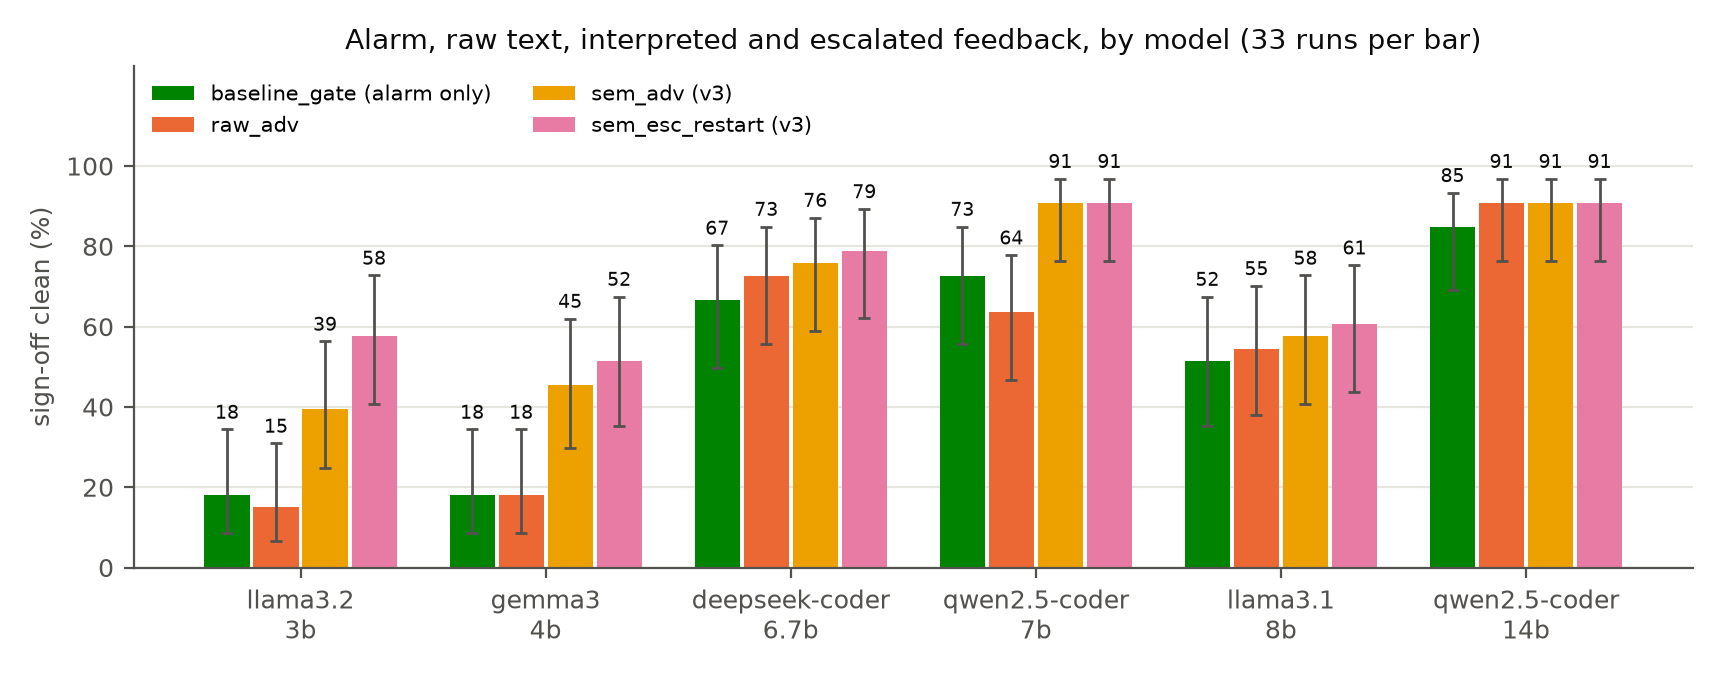
\includegraphics[width=\linewidth]{fig_p3_v2_by_model.png}
\caption{Sign-off clean per model under the alarm alone, raw tool text, v3 and
escalation ($33$ runs per bar, Wilson $95\%$ CI).}
\label{fig:s-p3-models}
\end{figure}

\begin{table}[htbp]
\centering
\caption{Re-stated contrasts on sign-off clean, six models (loop-clean value in
the last column).}
\label{tab:s-p3-restated}
\small
\begin{tabular}{@{}l l c c c@{}}
\toprule
\textbf{A $-$ B} & \textbf{Tasks} & \textbf{$\Delta$ [CI]} & \textbf{$p$} & \textbf{Loop-clean} \\
\midrule
\cond{sem\_adv} (v3) $-$ \cond{raw\_adv}          & all         & $+14.1$ [$+3.5$, $+24.7$]  & $0.014$    & $+14.6$ \\
                                                 & sim-silent  & $+20.4$ [$+5.6$, $+35.2$]  & $0.016$    & $+16.7$ \\
                                                 & sim-visible & $+6.7$ [$-7.8$, $+21.1$]   & $0.474$    & $+12.2$ \\
\cond{sem\_adv} (v2) $-$ \cond{raw\_adv}          & all         & $+10.1$ [$+2.0$, $+18.7$]  & $0.030$    & $+9.1$ \\
\cond{sem\_adv} (v3) $-$ \cond{sem\_adv} (v2)     & all         & $+4.0$ [$-4.0$, $+12.1$]   & $0.408$    & $+5.6$ \\
\cond{sem\_esc\_restart} $-$ \cond{sem\_adv} (v3) & all         & $+5.1$ [$-2.0$, $+12.6$]   & $0.255$    & $+6.1$ \\
\cond{sem\_esc\_restart} $-$ \cond{raw\_adv}      & all         & $+19.2$ [$+9.6$, $+28.8$]  & ${<}0.001$ & $+20.7$ \\
\cond{sem\_esc\_restart} $-$ \cond{baseline}      & sim-visible & $+14.4$ [$+3.3$, $+27.8$]  & $0.048$    & $+23.3$ \\
\bottomrule
\end{tabular}
\end{table}

\begin{table}[htbp]
\centering
\caption{Cost per condition, six models. Tool rounds: model calls whose prompt
carried tool feedback.}
\label{tab:s-p3-cost}
\small
\fitbox{\begin{tabular}{@{}l r r r r r@{}}
\toprule
\textbf{Condition} & \textbf{Calls/run} & \textbf{Tool rounds/run} & \textbf{Tokens/run} & \textbf{Tokens per sign-off clean} & \textbf{Clean by call 1} \\
\midrule
\cond{baseline}               & $1.34$ & $0.00$ & $1{,}425$ & $6{,}562$ & $15\%$ \\
\cond{raw\_adv}               & $3.27$ & $3.27$ & $4{,}396$ & $8{,}370$ & $41\%$ \\
\cond{sem\_adv} (v2)          & $2.83$ & $2.83$ & $3{,}831$ & $6{,}117$ & $46\%$ \\
\cond{sem\_adv} (v3)          & $2.51$ & $2.51$ & $3{,}377$ & $5{,}066$ & $55\%$ \\
\cond{sem\_esc\_restart} (v3) & $2.99$ & $1.32$ & $3{,}798$ & $5{,}295$ & $42\%$ \\
\cond{baseline\_gate}         & $3.39$ & $0.00$ & $3{,}835$ & $7{,}372$ & $40\%$ \\
\bottomrule
\end{tabular}}
\end{table}

\textbf{Per model, v3 minus raw text:} $+24.2$ (llama3.2:3b, $13/33$ against
$5/33$), $+27.3$ (gemma3:4b, $15/33$ against $6/33$), $+3.0$
(deepseek-coder:6.7b, $25$ against $24$), $+27.3$ (qwen2.5-coder:7b, $30$ against
$21$), $+3.0$ (llama3.1:8b, $19$ against $18$), $0$ (qwen2.5-coder:14b, $30$
each).

\begin{table}[htbp]
\centering
\caption{Sign-off clean per task, $k/18$ (six models $\times$ three replicates);
loop-clean in brackets where it differs.}
\label{tab:s-p3-task}
\small
\begin{tabular}{@{}l c c c c c c@{}}
\toprule
\textbf{Task} & \cond{baseline} & \cond{raw\_adv} & \textbf{v2} & \textbf{v3} & \textbf{esc (v3)} & \textbf{gate} \\
\midrule
\multicolumn{7}{@{}l}{\emph{Sim-silent}} \\
MuxPC             & $0$  & $17$ & $18$ & $18$ & $18$ & $15$ \\
execute\_mux      & $0$  & $10$ & $15$ & $15$ & $17$ & $12$ \\
mem\_wb\_mux      & $0$  & $9$ [$15$] & $11$ [$14$] & $11$ [$13$] & $11$ [$16$] & $9$ [$15$] \\
mux3              & $0$  & $12$ & $18$ & $18$ & $17$ & $12$ \\
register\_1bit    & $0$  & $10$ & $12$ & $15$ & $16$ & $10$ \\
riscv\_alu\_flags & $0$  & $6$  & $9$  & $9$  & $7$  & $3$ \\
\midrule
\multicolumn{7}{@{}l}{\emph{Sim-visible}} \\
Address\_select   & $0$ [$3$] & $1$ [$8$] & $1$ [$9$] & $2$ [$14$] & $4$ [$15$] & $0$ [$2$] \\
register\_32bit   & $15$ & $11$ & $12$ & $15$ & $16$ & $14$ \\
register\_4bit    & $14$ & $10$ & $11$ & $14$ & $17$ & $15$ \\
noc\_xbar4        & $10$ & $9$  & $10$ & $9$  & $9$  & $9$ \\
ni\_flit\_pack    & $4$  & $9$  & $7$  & $6$  & $10$ & $4$ \\
\bottomrule
\end{tabular}
\end{table}

\begin{table}[htbp]
\centering
\caption{Where v2 was silent or misleading. Fired: runs with a directive on the
defective input ($/18$). Clean: sign-off clean ($/18$), loop-clean in brackets
where it differs.}
\label{tab:s-p3-upgrade}
\small
\begin{tabular}{@{}l l c c c c@{}}
\toprule
\textbf{Task} & \textbf{v2 on the input} & \textbf{v2 fired} & \textbf{v3 fired} & \textbf{v2 clean} & \textbf{v3 clean} \\
\midrule
register\_1bit  & silent (abort unhandled)        & $0$  & $18$ & $12$ & $15$ \\
ni\_flit\_pack  & silent (expression truncation)  & $0$  & $18$ & $7$  & $6$ \\
register\_32bit & gate on the clock (misleading)  & $18$ & $18$ & $12$ & $15$ \\
register\_4bit  & gate on the clock (misleading)  & $18$ & $18$ & $11$ & $14$ \\
Address\_select & extra gating directive on a bus & $18$ & $18$ & $1$ [$9$] & $2$ [$14$] \\
\bottomrule
\end{tabular}
\end{table}

\textbf{Escalation.} $142/198$ sign-off clean ($72\%$), $1.32$ tool rounds per
run against $2.51$ for always-on v3 ($47.5\%$ fewer). On sim-visible tasks
deepseek-coder:6.7b reaches $13/15$ and qwen2.5-coder:7b $12/15$ against
baseline's $9/15$ each. $109$ runs never escalated ($100$ ended sign-off clean);
the $89$ that did ended $42$ sign-off clean.

\begin{table}[htbp]
\centering
\caption{Top-level synthesis pass after splicing in each condition's repaired
leaves ($18$ groups per cell, six models), and in brackets the groups that also
reach the golden latch bound.}
\label{tab:s-p3-compose}
\small
\begin{tabular}{@{}l c c c c c c@{}}
\toprule
\textbf{Design} & \cond{baseline} & \cond{raw\_adv} & \textbf{v2} & \textbf{v3} & \textbf{esc (v3)} & \textbf{gate} \\
\midrule
$2{\times}2$ mesh & $0$ ($0$) & $15$ ($10$) & $13$ ($11$) & $16$ ($15$) & $18$ ($16$) & $11$ ($8$) \\
$3{\times}3$ mesh & $0$ ($0$) & $15$ ($10$) & $13$ ($11$) & $16$ ($15$) & $18$ ($16$) & $11$ ($8$) \\
MPSoC top         & $0$ ($0$) & $13$ ($8$)  & $12$ ($8$)  & $16$ ($14$) & $15$ ($13$) & $11$ ($1$) \\
\bottomrule
\end{tabular}
\end{table}

\begin{figure}[htbp]
\centering
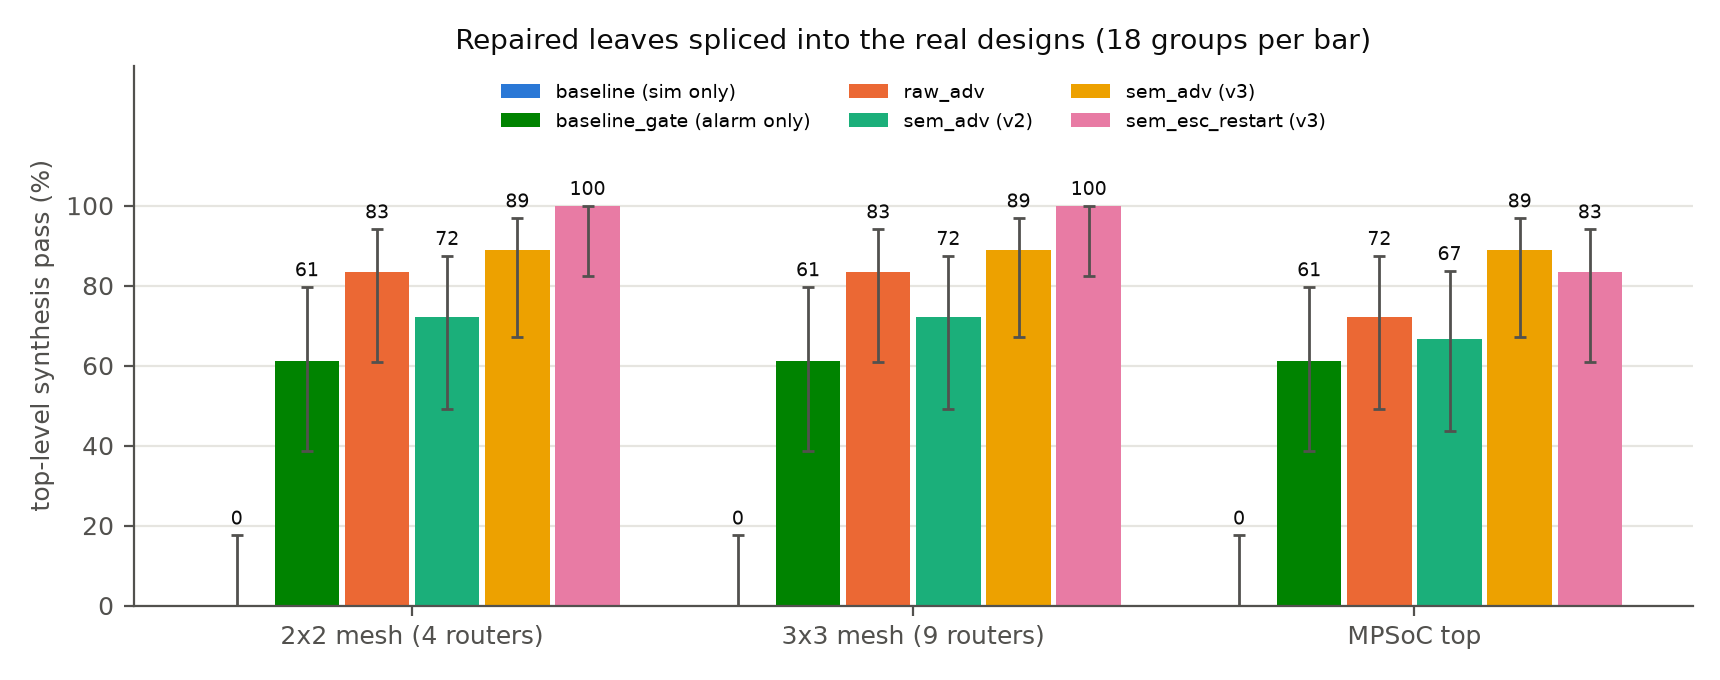
\includegraphics[width=0.9\linewidth]{fig_p3_v2_composition.png}
\caption{Top-level synthesis pass of the two meshes and the MPSoC after
splicing in repaired leaves, by condition (Wilson $95\%$ CI).}
\label{fig:s-p3-compose}
\end{figure}

For qwen2.5-coder:32b every tool condition composes $3/3$ at the bound in all
three designs, and baseline $0/3$.

\subsection{Oracle integrity}

Every clean repair of the $990$ runs was checked against the golden fix with
Yosys (\texttt{equiv\_make}, \texttt{equiv\_simple -seq 5},
\texttt{equiv\_induct}), and its constant-driven output bits were counted; each
golden fix is equivalent to itself. Where a candidate was not proven equivalent,
the check was repeated with inputs the specification declares illegal mapped to
a legal value. No clean repair ties an output bit to a constant beyond the golden
fix. On MuxPC, execute\_mux, mux3, register\_1bit and riscv\_alu\_flags every clean
repair is equivalent, or equivalent on legal inputs.

\begin{table}[htbp]
\centering
\caption{Equivalence audit of the clean runs (all conditions of the $990$ runs).
Class (i): differs from the golden fix on behaviour the specification defines and
the loop testbench does not check.}
\label{tab:s-p3-audit}
\small
\begin{tabular}{@{}l c c c c@{}}
\toprule
\textbf{Task} & \textbf{Clean runs} & \textbf{Equivalent} & \textbf{Equivalent on legal inputs} & \textbf{Class (i)} \\
\midrule
Address\_select  & $49$ & $8$  & $0$  & $41$ \\
ni\_flit\_pack   & $36$ & $36$ & $0$  & $0$ \\
noc\_xbar4       & $47$ & $0$  & $47$ & $0$ \\
register\_32bit  & $69$ & $69$ & $0$  & $0$ \\
register\_4bit   & $66$ & $66$ & $0$  & $0$ \\
mem\_wb\_mux     & $58$ & $42$ & $0$  & $16$ \\
\bottomrule
\end{tabular}
\end{table}

For each gap the sign-off testbench passes the golden fix, fails every class-(i)
repair, still passes every other clean repair, and fails a golden mutant that
differs only in the unchecked cases.

\begin{table}[htbp]
\centering
\caption{Gap runs (loop-clean, failing sign-off), six models, and how many
received the production latch text (``\texttt{<safe value>}'' at the top of the
block) in any feedback round. A count, not a causal claim.}
\label{tab:s-p3-advice}
\small
\begin{tabular}{@{}l c c c c c c@{}}
\toprule
 & \cond{baseline} & \cond{raw\_adv} & \textbf{v2} & \textbf{v3} & \textbf{esc (v3)} & \textbf{gate} \\
\midrule
Address\_select: gap runs       & $3$ & $7$ & $8$ & $12$ & $11$ & $2$ \\
\quad with the advice           & $0$ & $0$ & $8$ & $12$ & $11$ & $0$ \\
mem\_wb\_mux: gap runs          & $0$ & $6$ & $3$ & $2$  & $5$  & $6$ \\
\quad with the advice           & $0$ & $0$ & $3$ & $2$  & $0$  & $0$ \\
\bottomrule
\end{tabular}
\end{table}

On \texttt{mem\_wb\_mux} the same advice also reached every v2 and v3 run that
ended sign-off clean ($11/11$ each).

\subsection{Up the ladder}

\begin{table}[htbp]
\centering
\caption{Ladder rows ($33$ runs per cell, $N{=}3$; not pooled): sign-off clean as
sim-silent (of $18$) $+$ sim-visible (of $15$), and tokens per run.}
\label{tab:s-p3-ladder}
\footnotesize
\setlength{\tabcolsep}{3.5pt}
\begin{tabular}{@{}l cr cr cr cr@{}}
\toprule
 & \multicolumn{2}{c}{\textbf{qwen2.5-coder:32b}} & \multicolumn{2}{c}{\textbf{gpt-4.1-mini}} & \multicolumn{2}{c}{\textbf{claude-haiku-4.5}} & \multicolumn{2}{c}{\textbf{gemini-2.5-flash}} \\
\cmidrule(lr){2-3}\cmidrule(lr){4-5}\cmidrule(lr){6-7}\cmidrule(l){8-9}
\textbf{Condition} & clean & tokens & clean & tokens & clean & tokens & clean & tokens \\
\midrule
\cond{baseline}               & $0{+}12$  & $663$     & $0{+}12$  & $440$     & $0{+}12$  & $517$     & $0{+}15$  & $516$ \\
\cond{baseline\_gate}         & $16{+}12$ & $1{,}824$ & $16{+}12$ & $1{,}529$ & $18{+}12$ & $1{,}099$ & $18{+}15$ & $1{,}160$ \\
\cond{raw\_adv}               & $18{+}12$ & $1{,}492$ & $18{+}12$ & $1{,}164$ & $18{+}12$ & $1{,}334$ & $18{+}12$ & $1{,}291$ \\
\cond{sem\_adv} (v2)          & $18{+}12$ & $1{,}655$ & $18{+}12$ & $1{,}255$ & $18{+}12$ & $1{,}517$ & $18{+}15$ & $1{,}478$ \\
\cond{sem\_adv} (v3)          & $18{+}12$ & $1{,}660$ & $18{+}12$ & $1{,}257$ & $18{+}12$ & $1{,}524$ & $18{+}14$ & $1{,}479$ \\
\cond{sem\_esc\_restart} (v3) & $18{+}12$ & $1{,}850$ & $18{+}12$ & $1{,}404$ & $18{+}12$ & $1{,}101$ & $18{+}15$ & $1{,}225$ \\
\bottomrule
\end{tabular}
\end{table}

\begin{figure}[htbp]
\centering
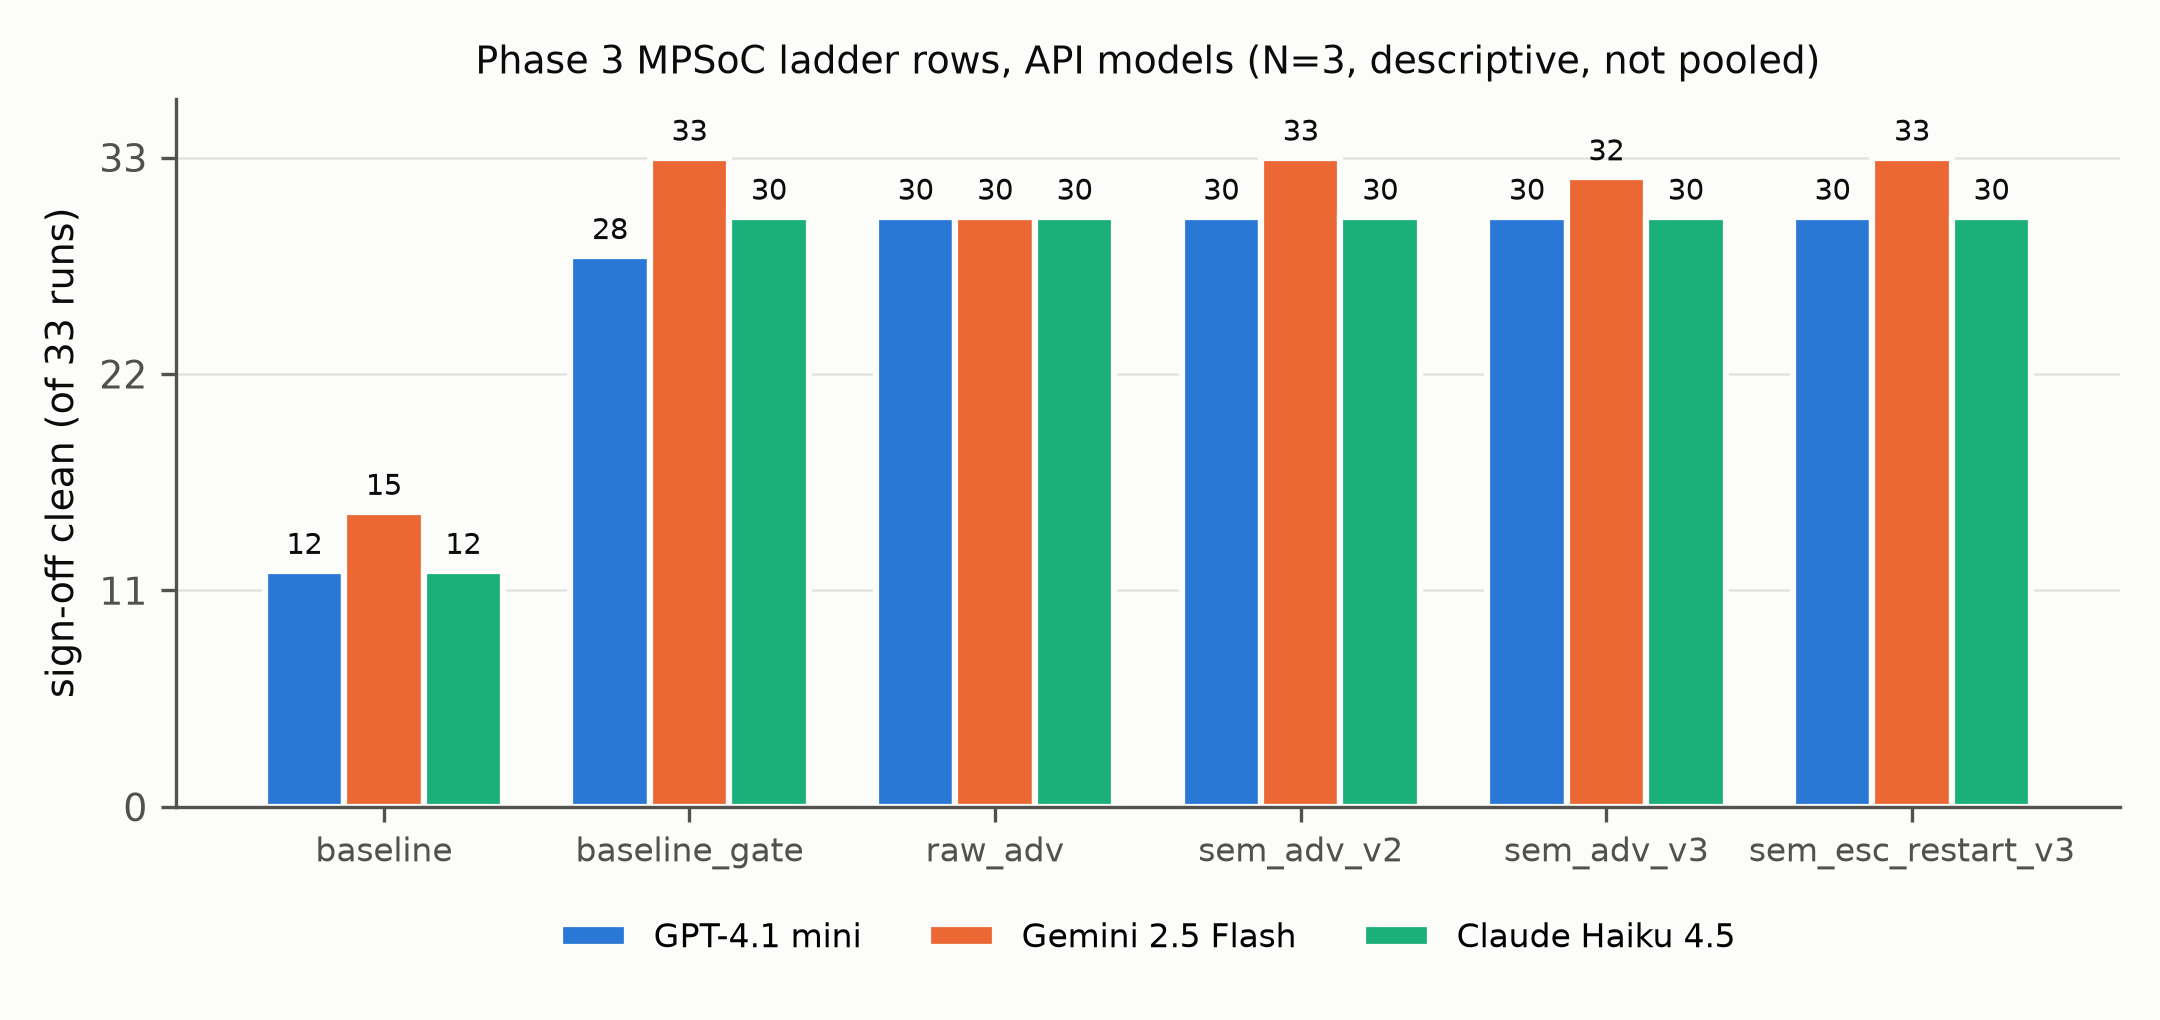
\includegraphics[width=0.8\linewidth]{fig_p3_api_ladder_signoff.png}
\caption{The three API ladder rows: sign-off clean of $33$ by condition.}
\label{fig:s-p3-api}
\end{figure}

Every non-baseline miss of the three API models is on Address\_select, apart from
two alarm-only runs on riscv\_alu\_flags for GPT-4.1 mini; Gemini~2.5 Flash's
misses are raw text ($3$ of $3$) and v3 ($1$ of $3$). In the seven-model
sensitivity pool (six models plus qwen2.5-coder:32b) every contrast keeps its
sign: escalation minus the alarm $+17.7$ (CI $+10.4$ to $+25.6$), v3 minus the
alarm $+13.4$ (CI $+3.5$ to $+23.8$).

\subsection{Next steps from the case study}

Held-out defects for the v3 rules; a specification-valued default in the latch
directive; returning the best candidate so far (some runs pass simulation at some
point and lose it: $23$ of $198$ under v3 and $11$ under escalation in the $990$
runs); more replicates on the flat tasks (\texttt{noc\_xbar4},
\texttt{riscv\_alu\_flags}); and integration-level feedback.

% ============================================================================
\section{Statistics and Reproducibility}
\label{s:stats}

Rates carry Wilson $95\%$ intervals. Paired contrasts match runs on (model, task
or module, replicate); runs are independent draws, so the matching is a
stratification. Because the replicates of a cell are correlated, general claims
use the mean over cells of the within-cell rate difference, with a cell bootstrap
($10{,}000$ resamples, percentile interval) and a two-sided sign-flip
permutation test over cells ($20{,}000$ random sign patterns,
$p = (1 + \#\{|\bar d^{*}| \geq |\bar d|\}) / 20{,}001$), both seeded per label
(seed $20260925$ and the CRC of the label), so reruns reproduce byte for byte. The Set~4 copy of
these functions reproduces all twelve published Set~1 and Set~3 values exactly
before any contrast is reported. Per-model and per-task Phase~3 breakdowns use
run-level McNemar tests with Holm correction within each contrast. The deficit
figure uses Newcombe intervals for a difference of two independent proportions.

Every table and figure can be regenerated from the repository; the commands and
the canonical evidence file for each section are listed in \texttt{REPO\_INDEX.md}.

\end{document}
